\begin{center}
  \textbf{Отчёт лабораторной работы №\envReportLabNumber}
\end{center}

\textbf{Тема}:
<<\envReportTitle>>

\textbf{Цель}:
изучить основы метода опорных векторов (support vector machine, SVM) в
контексте задачи классификации, приобрести навыки работы с методом SVM в
системе STATISTICA StatSoft, осуществить обработку методом SVM
индивидуального набора данных и интерпретацию результатов.
% = = = = = = = = = = = = = = = =

\begin{center}
  \textbf{Ход работы}
\end{center}

Удаляю папку <<Statistica 10 RUS>> (тут временные файлы portable программы).

Запускаю Ststatistica\_10\_ru\_portable.exe.

\begin{center}
  \textbf{Файл данных}
\end{center}

Главная > Открыть > IrisSNN.sta > Открыть

Результат на рисунке~\ref{fig:1}.

\begin{figure}[!h]
  \centering

  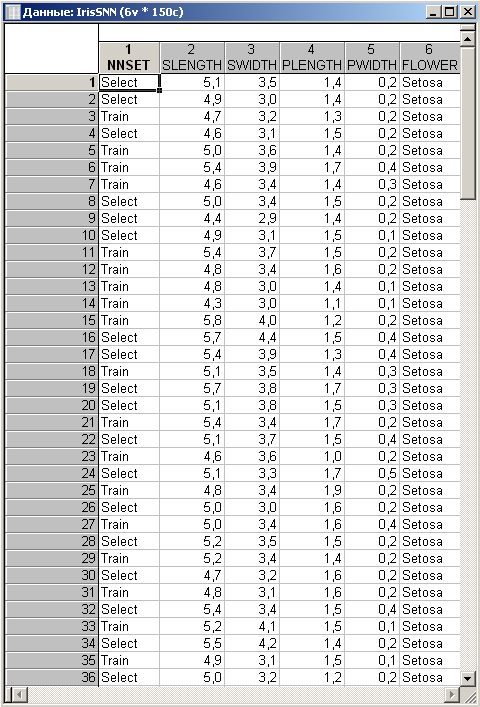
\includegraphics[height=15cm]
  {inc/ex_1.PNG}

  \caption{1}

  \label{fig:1}
\end{figure}

\newpage

\begin{center}
  \textbf{Запуск анализа}
\end{center}

Добыча данных > Процедуры обучения > Support Vector Machine > OK

Результаты на рисунках~\ref{fig:2} и \ref{fig:3}.

\begin{figure}[!h]
  \centering

  \begin{minipage}{0.49\textwidth}
    \centering

    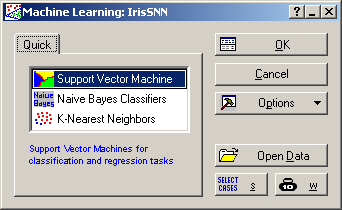
\includegraphics[height=5cm]
    {inc/ex_2.PNG}

    \caption{2}

    \label{fig:2}
  \end{minipage}
  \begin{minipage}{0.49\textwidth}
    \centering

    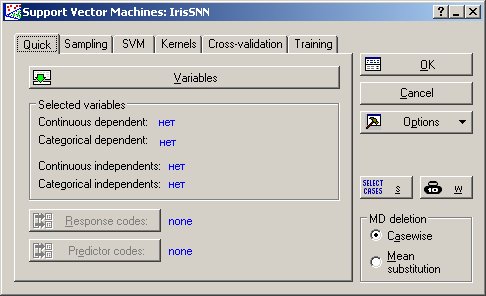
\includegraphics[height=5cm]
    {inc/ex_3.PNG}

    \caption{3}

    \label{fig:3}
  \end{minipage}
\end{figure}

\begin{center}
  \textbf{Настройки анализа}
\end{center}

> Быстрый > Variables \\
> Categorical dependents > 6-FLOWER \\
> Continuous predictors > 2 > Shift > 5 \\
> OK

Результат на рисунке~\ref{fig:4}.

\begin{figure}[!h]
  \centering

  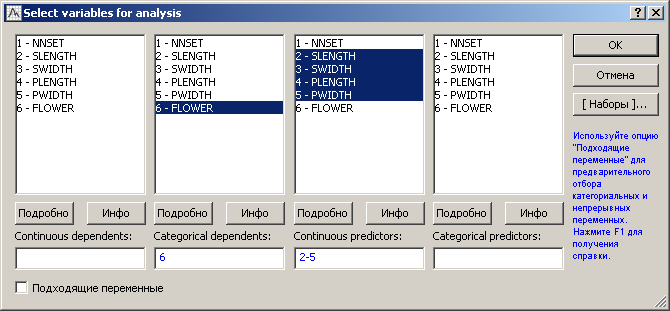
\includegraphics[width=12cm]
  {inc/ex_4.PNG}

  \caption{4}

  \label{fig:4}
\end{figure}

> Sampling > Use sample variable > Sample \\
> Sample Identifier Variable > 1-NNSET > OK \\
> Status > On \\
> Code for analysis sample (2 раза клик) > 102:Train > OK > OK

Результаты на рисунках~\ref{fig:5}, \ref{fig:6}, \ref{fig:7},
\ref{fig:8}, \ref{fig:9}, \ref{fig:10}.

\begin{figure}[!h]
  \centering

  \begin{minipage}{0.32\textwidth}
    \centering

    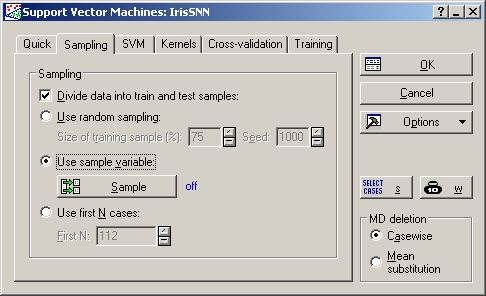
\includegraphics[height=3.8cm]
    {inc/ex_5.PNG}

    \caption{5}

    \label{fig:5}
  \end{minipage}
  \begin{minipage}{0.42\textwidth}
    \centering

    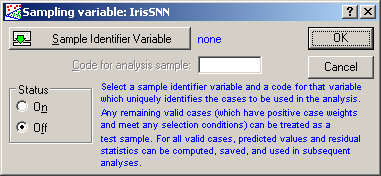
\includegraphics[width=5cm]
    {inc/ex_6.PNG}

    \caption{6}

    \label{fig:6}
  \end{minipage}
  \begin{minipage}{0.22\textwidth}
    \centering

    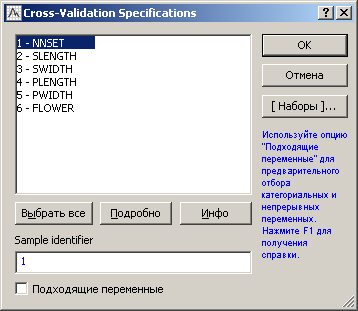
\includegraphics[height=3.8cm]
    {inc/ex_7.PNG}

    \caption{7}

    \label{fig:7}
  \end{minipage}
\end{figure}

\begin{figure}[!h]
  \centering

  \begin{minipage}{0.32\textwidth}
    \centering

    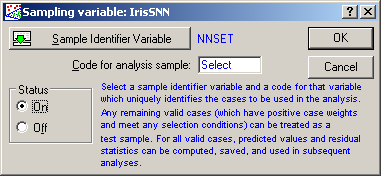
\includegraphics[width=6cm]
    {inc/ex_8.PNG}

    \caption{8}

    \label{fig:8}
  \end{minipage}
  \begin{minipage}{0.32\textwidth}
    \centering

    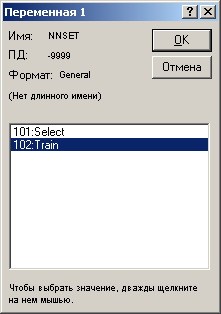
\includegraphics[height=3.8cm]
    {inc/ex_9.PNG}

    \caption{9}

    \label{fig:9}
  \end{minipage}
  \begin{minipage}{0.32\textwidth}
    \centering

    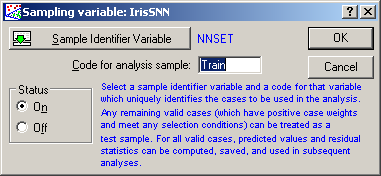
\includegraphics[width=6cm]
    {inc/ex_10.PNG}

    \caption{10}

    \label{fig:10}
  \end{minipage}
\end{figure}

\newpage

> Cross-validation > Apply v-fold cross-validation > OK

Результаты на рисунках~\ref{fig:11}, \ref{fig:12}.

\begin{figure}[!h]
  \centering

  \begin{minipage}{0.49\textwidth}
    \centering

    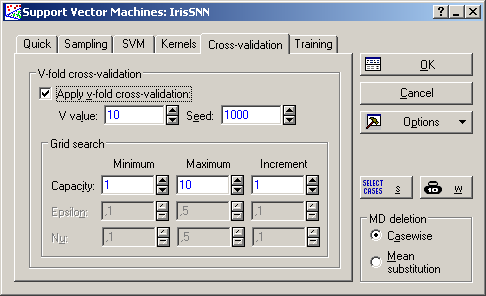
\includegraphics[height=6cm]
    {inc/ex_11.PNG}

    \caption{11}

    \label{fig:11}
  \end{minipage}
  \begin{minipage}{0.49\textwidth}
    \centering

    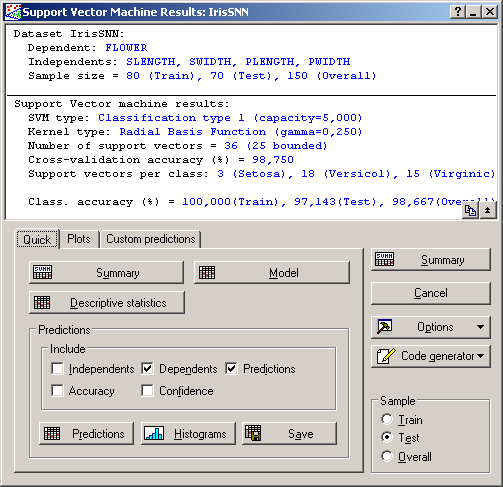
\includegraphics[height=6cm]
    {inc/ex_12.PNG}

    \caption{12}

    \label{fig:12}
  \end{minipage}
\end{figure}

\begin{center}
  \textbf{Просмотр результатов}
\end{center}

> Summary

Результат на рисунке~\ref{fig:13}.

\begin{figure}[!h]
  \centering

  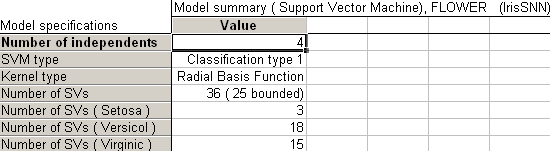
\includegraphics[height=2.5cm]
  {inc/ex_13.PNG}

  \caption{13}

  \label{fig:13}
\end{figure}

\newpage

\begin{center}
  \textbf{Примечание}
\end{center}

Support Vector Machine Results: IrisSNN > Quick > Model

Результат на рисунке~\ref{fig:14}.

\begin{figure}[!h]
  \centering

  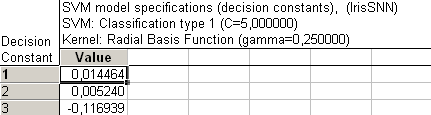
\includegraphics[height=3cm]
  {inc/ex_14.PNG}

  \caption{14}

  \label{fig:14}
\end{figure}

Support Vector Machine Results: IrisSNN > Quick > Descriptive statistics

Результат на рисунке~\ref{fig:15}.

\begin{figure}[!h]
  \centering

  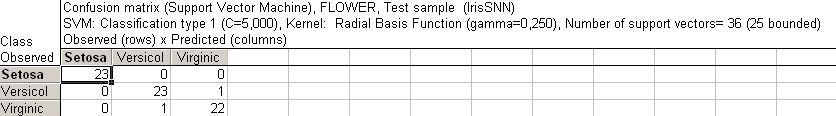
\includegraphics[width=18cm]
  {inc/ex_15.PNG}

  \caption{15}

  \label{fig:15}
\end{figure}

Support Vector Machine Results: IrisSNN > Quick > Include \\
> (Independents, Dependents, Predictions, Accuracy, Confidence) \\
> Predictions

Результаты на рисунках~\ref{fig:16}, \ref{fig:17}, \ref{fig:18}.

\begin{figure}[!h]
  \centering

  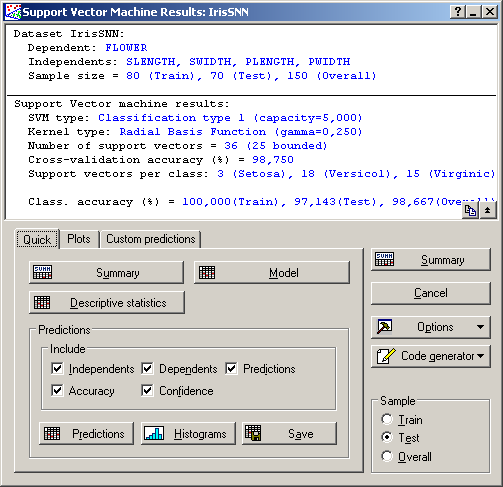
\includegraphics[height=9cm]
  {inc/ex_16.PNG}

  \caption{16}

  \label{fig:16}
\end{figure}

\begin{figure}[!hp]
  \centering

  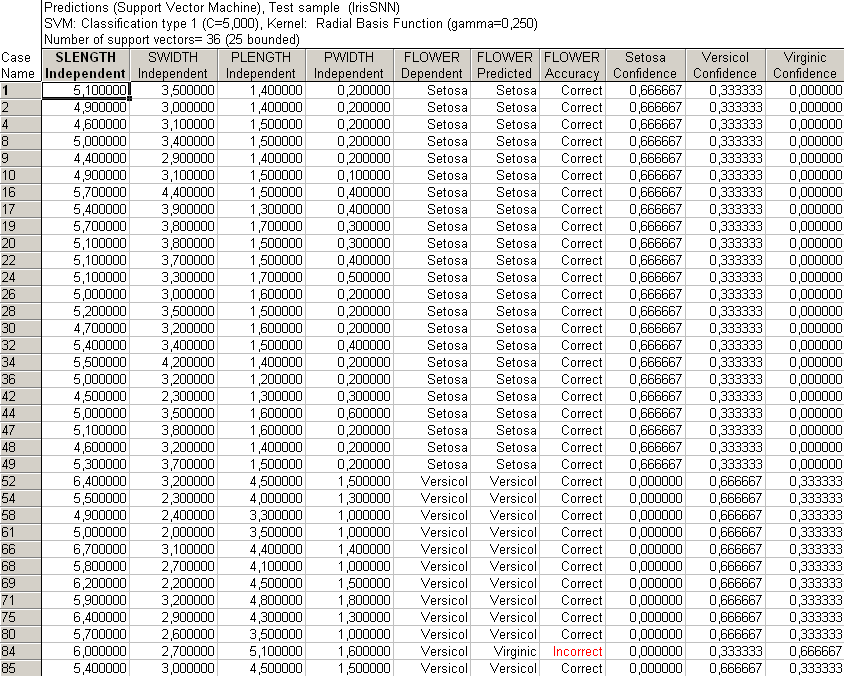
\includegraphics[width=14cm]
  {inc/ex_17.PNG}

  \caption{17}

  \label{fig:17}
\end{figure}

\begin{figure}[!hp]
  \centering

  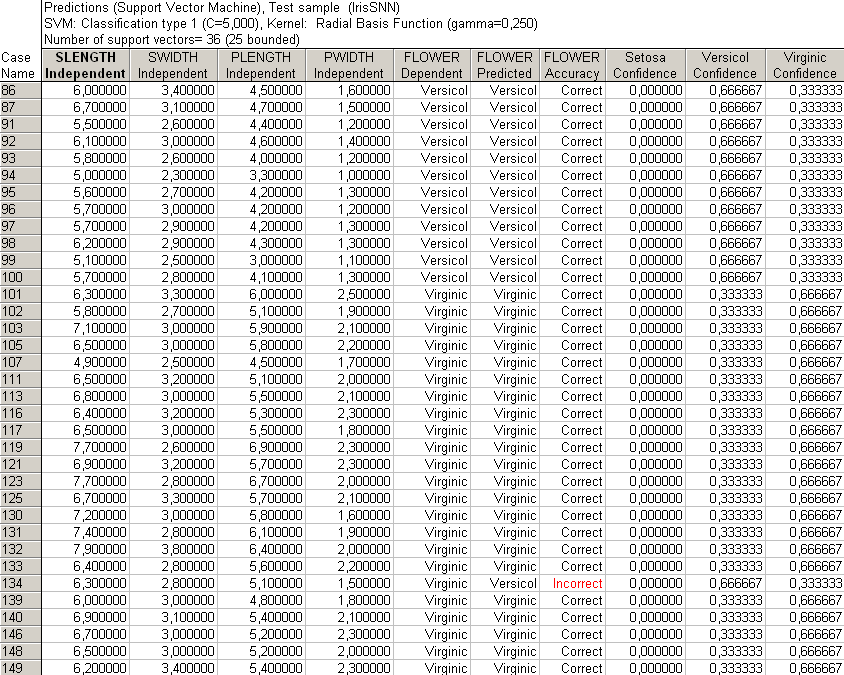
\includegraphics[width=14cm]
  {inc/ex_18.PNG}

  \caption{18}

  \label{fig:18}
\end{figure}

\newpage

Support Vector Machine Results: IrisSNN > Plots \\
> X-axis > PLENGTH \\
> Y-axis > Sentosa (conf.) > Ctrl > Versicol (conf.) > Ctrl > Virginic (conf.) \\
> Graphs of X and Y

Результаты на рисунках~\ref{fig:19}, \ref{fig:20}.

\begin{figure}[!h]
  \centering

  \begin{minipage}{0.49\textwidth}
    \centering

    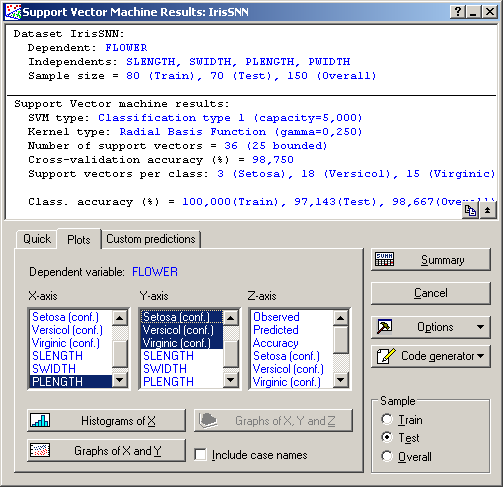
\includegraphics[height=7cm]
    {inc/ex_19.PNG}

    \caption{19}

    \label{fig:19}
  \end{minipage}
  \begin{minipage}{0.49\textwidth}
    \centering

    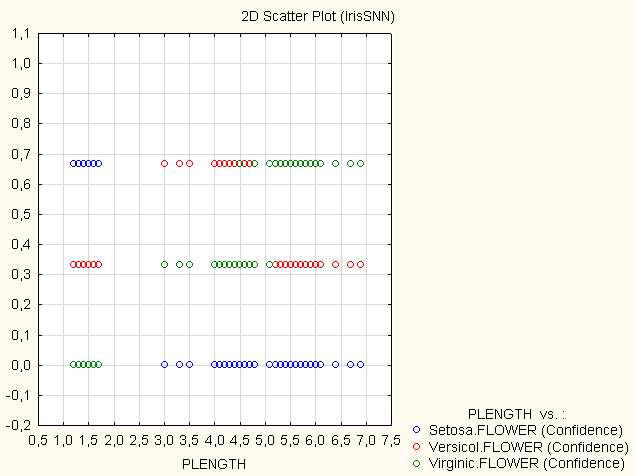
\includegraphics[height=7cm]
    {inc/ex_20.PNG}

    \caption{20}

    \label{fig:20}
  \end{minipage}
\end{figure}

Support Vector Machine Results: IrisSNN > Custom predictions > User defined case \\
> SLENGTH > 7 \\
> SWIDTH > 5 \\
> PLENGTH > 8 \\
> PWIDTH > 3 \\
> OK > Predictions

Результаты на рисунках~\ref{fig:21}, \ref{fig:22}, \ref{fig:23}, \ref{fig:24}.

\begin{figure}[!h]
  \centering

  \begin{minipage}{0.49\textwidth}
    \centering

    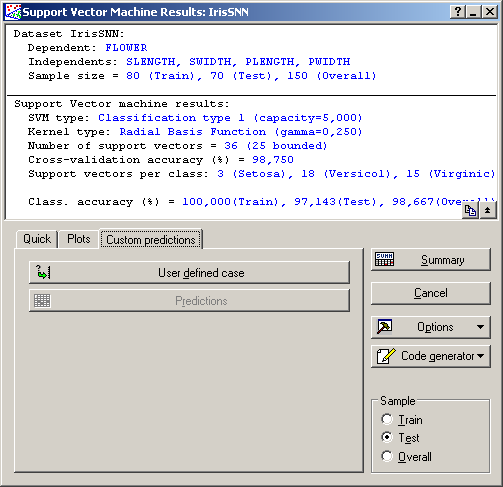
\includegraphics[height=7cm]
    {inc/ex_21.PNG}

    \caption{21}

    \label{fig:21}
  \end{minipage}
  \begin{minipage}{0.49\textwidth}
    \centering

    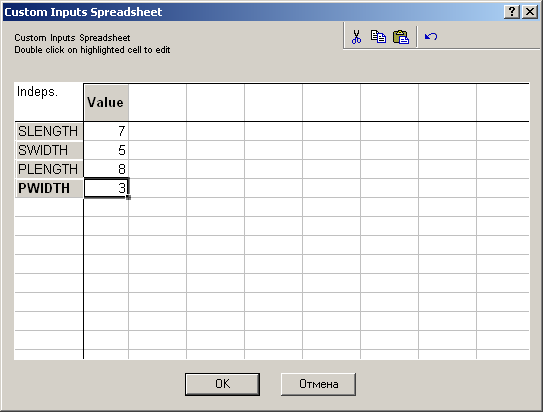
\includegraphics[height=7cm]
    {inc/ex_22.PNG}

    \caption{22}

    \label{fig:22}
  \end{minipage}
\end{figure}

\begin{figure}[!h]
  \centering

  \begin{minipage}{0.49\textwidth}
    \centering

    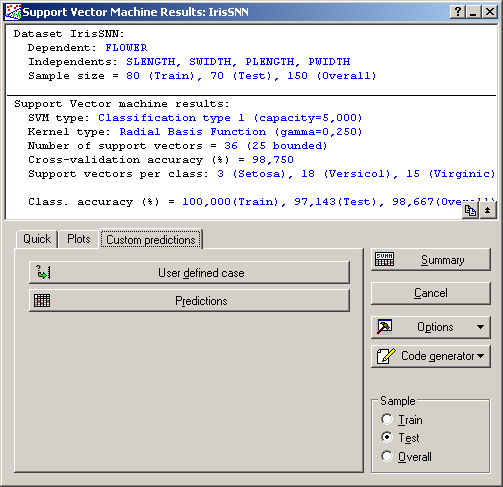
\includegraphics[height=7cm]
    {inc/ex_23.PNG}

    \caption{23}

    \label{fig:23}
  \end{minipage}
  \begin{minipage}{0.49\textwidth}
    \centering

    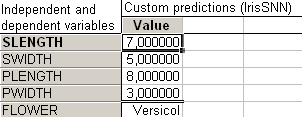
\includegraphics[width=8cm]
    {inc/ex_24.PNG}

    \caption{24}

    \label{fig:24}
  \end{minipage}
\end{figure}

\newpage

\begin{center}
  \textbf{Вариант 5}
\end{center}
